\section{Results}
\label{sec:results}




\newcommand{\ans}[1]{\underline{\textbf{Answer~#1:}}}


 
 
  \begin{table} 
  \caption{Median performance improvements seen after applying all the treatments A1 (defined in \S\ref{rx}); i.e. all of
{\em instance}, {\em label}, {\em boundary}  and {\em parameter} engineering.}
 \begin{center}
{\scriptsize  \begin{tabular}{|c|c|c|c|c|}\cline{3-5} 
    \multicolumn{2}{c|}{} &       &  From right-& \\ 
    \multicolumn{2}{c|}{} & From     &  hand-side & \\  
     \multicolumn{2}{c|}{} &   Table~\ref{tab:initial_svm}  &  of Table~\ref{tab:results} &  Improvement \\\hline
                             & precision   & 50 & 100 & 50\\ 
{\em higher} is {\em better} & AUC         &  41& 90 & 59\\ 
                             & recall      &  19 & 100 & 89\\\hline
{\em lower} is {\em better}  & false alarm & 32 & 0 & 32\\\hline
\end{tabular}} 
\end{center}
\label{summary}
\end{table}
  
  
  
 

% Given the large improvements seen after apply our treta  large improvements seen in Table~\ref{summary} conjectured that learners fault to predict actionable
% static code warnings if they must negotiate a complex decision landscape. 

% o remove the ``bumpiness'' in data like Figure~\ref{fig:loss}, we need to 
% pull and push the decision boundaries between different classes into a smoother shape.
% But also, unlike simplistic $(C,\gamma)$ tuning available in radial  SVMs, we want that process to perform differently
% in different parts of the data.


The results of the Table~\ref{tab:treatments} treatments are shown in   Table~\ref{tab:results}
(and 
another brief summary is offered in
Table~\ref{summary}).
These results are somewhat
extensive
  so, by way of an overview, we offer the following summary tool.
 The cells shown in  \colorbox{pink}{pink} are those that are   worse than the A1 results 
  (and A1 is our recommended GHOST2 method). 
 Looking over those pink cells
 we can see that across our data sets and across our different measures, our recommend method (A1) does as well (or better) than anything else. 
 
 (Technical aside: looking at this pink cells, it could be said that   A5 comes close to A1, but A5 loses a little on recalls).
 Nevertheless, we have strong reasons for recommending A1 over A5 since, recalling Table~\ref{tab:treatments},
 A5 requires a labelling for 100\% of the data. On the other hand A1, that uses label engineering,
 achieves its results using 10\% of the labels. This is important since, as  said in our introduction, 
one way to address, in part, the methodological problems
raised by Kang et al. GHOST2 makes its conclusions
using a small percentage of the raw data (10\%). That is,
to address to issues of corrupt data found by Kang et
al., we say ``use less data'' and, for the data that is used,
``reflect more on that data''.)
 
 Using these results,
we can answer our research questions as follows. 
 


\subsection*{ \rqn{1} For detecting actionable static code warnings,
what data mining methods should we recommend?}
  

Regarding feedforward networks versus, say,  traditional learners (decision trees, random forests, logistic regression and SVMs), the traditional learners all performed worse than the 
feedforward networks used in treatment A1 (evidence: compare treatments
A1 with A7 which use feedforward or traditional learners, respectively; there are four perfect AUCs
for feedforward networks in A1, i.e AUC=100\%, but only two for the A7 results). 



As to why 
the 1980s style
feedforward networks worked better than newer neural net technology,  we note that feedforward networks run so fast
than it is easier to extensively tune them. Perhaps
 (a)~faster learning plus (b)~more tuning might lead to better results
that then non-linear modeling of an off-the-shelf learner.
This could be an interesting avenue for future work.

As to the value of {\em boundary, label, instance}
and {\em parameter} engineering,   in the ablation study, removing any of these led to worse results.
For example, 
with {\em boundary engineering},
   A1
(that uses boundary engineering) generates more perfect
scores (e.g. AUC=100\%) than A4 (that does not use it).
Also, for recall, A1 always performed
as good or better than A4 in 6/8 data sets. Similarly, A4 suffers from a drop in AUC score across the board.

 
As for {\em label engineering}, from A1 to A5,
specializing our data to just 10\% of
the labels (in A1) yields nearly the same precisions
which using 100\% of the data (in A5) in nearly all the AUC results. Moreover, the AUC score for A1 is perfect in 4/8 cases, while for A5, it is rarely the case.



As to {\em instance engineering},
without it the  
precision can crash to zero
(compare A1 to A2, particularly  the smaller data sets) while often leading to
lower recalls. The smaller datasets also see a decrease in AUC for A2.


 
Measured in terms of false alarm, these results strongly recommend 
{\em parameter engineering}. Without parameter engineering, some of those treatments could find too many static code warnings and hence suffer from
excessive false alarms (evidence: see the A3 false alarm results in nearly every data set). A1 (which used all the   treatments of \S\ref{rx}) had lower false alarm rates than anything else (evidence: we rarely see the dark blue A1 spike in the false alarm results). The  only exception to the observation that ``parameter engineering leads to lower false alarm results''
are seen in the   DERBY
data set. That data set turns out to be particularly tricky in that, nearly always, modeling methods  that achieved low false alarm rates on that data set
also had to be satisfied with much lower recalls. 
 
 
\begin{figure}[!t]
   \begin{center}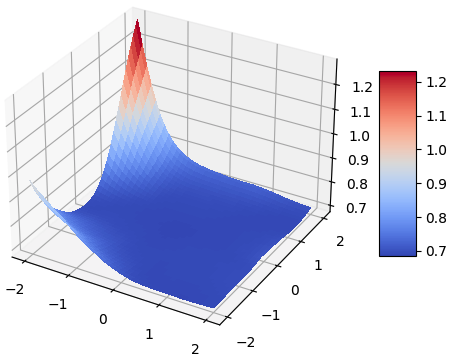
\includegraphics[width=.3\textwidth]{rahul/after.png} \end{center} 
    \caption{ Error landscape in the TOMCAT  after applying the treatments of \S\ref{rx}. To understand the simplifications achieved via our methods, the reader might find it insightful to  compare this figure against Figure~\ref{fig:loss}. }
    \label{fig:gain}
\end{figure}



One final point is that these results do not  recommend 
the use of certain widely used neural network
technologies such as CNN or CodeBERT for finding actionable
static code warnings.
CNN-based treatments (B2 and C2) suffer from low precision and AUC scores (see Table \ref{tab:results}).
Similarly, as shown Table~\ref{tab:results}, CodeBERT
often suffers from   low precision and poor false alarms
and (in the case of CodeBERT) some very low recalls indeed.


In summary:
\begin{formal}
\ans{1} To recognize actionable static code warnings, apply all the treatments of \S\ref{rx}. Also, 
spend most tuning faster feedforward neural nets  rather than trusting (a)~traditional learners or (b)~more recent
``bleeding edge'' neural net methods.
\end{formal}



  
 
\subsection*{\rqn{2} Does GHOST2's combination of instance, label, boundary
and parameter engineering, reduce the complexity of the
decision boundary?}

Previously, this paper argued
that reason for the poor performance
seen in prior was due to the complexity
of the data (specifically, the bumpy shape seen in  Figure~\ref{fig:loss}).
Our treatments of \S\ref{rx} were  designed to simplify that landscape. Did we succeed?

 Figure~\ref{fig:gain}
 shows the landscape in  TOMCAT after
 the   treatments of \S\ref{rx}
 were applied.
 By comparing this figure with
      Figure~\ref{fig:loss},
      we can see that our treatments
      achieved the desired goal
      of removing the ``bumps''.
      
 
 \begin{wraptable}{r}{1.7in}
     
    \caption{Percent changes in \citet{li2018visualizing}'s
    smoothness metric, seem after applying the methods of this paper.}
    \label{tab:fuzzy}
    \begin{tabular}{lr}
        \toprule
        \textbf{Dataset} & \textbf{\% change} \\
        \midrule
        
   \rowcolor{gray!15}       maven & 158.87 \\
        
        cassandra & 73.09 \\
        
        \rowcolor{gray!15}       jmeter & 55.53 \\
        tomcat & 36.34 \\
        \rowcolor{gray!15}       derby & 31.35 \\
        commons & 29.61 \\
         \rowcolor{gray!15}      ant & 24.78 \\
        lucene-solr & 16.46 \\
        \midrule
        \textbf{median} & \textbf{33.85} \\
        \bottomrule
    \end{tabular}
\end{wraptable}

 As to the other data
      sets,
      \citet{li2018visualizing}
      propose a ``smoothness'' equation
      to measure a data set's
      ``bumps''.
      Table~\ref{tab:fuzzy}
      shows the percentage 
      change in that smoothness
      measure seen   after applying the methods of this paper. 
       All these changes
    are positive, indicating that the resulting landscapes are much smoother.
    For an intuition of what these numbers mean,    the TOMCAT change of 36.35\% results in Figure \ref{fig:loss}  
    changing to Figure \ref{fig:gain}.
    
    Hence we say:
    
    
\begin{formal}
\ans{2} Label, parameter, instance and boundary engineering can simplify the
internal structure of   training
data.
\end{formal}





\subsection*{
\rqn{3}  Does  GHOST2's  combination of {\em instance}, {\em label}, {\em boundary}  and {\em parameter}  improve predictive performance?} 
     
   
 Table~\ref{summary} shows the performance
 improvements   after
 smoothing out our training
 data from (e.g.)
 Figure \ref{fig:loss} to 
 Figure \ref{fig:gain}. On 4/8 datasets, we achieve perfect scores. Moreover, we showed through an ablation study that each of the components of GHOST2 is necessary. For example, row A3 in Table \ref{tab:results} is another piece of evidence that hyper-parameter optimization is necessary. The feedforward networks of our approach outperformed more complex learners (CNNs and CodeBERT)--we refer the reader to rows B2, C2, and CodeBERT in Table \ref{tab:results}. On the other hand, going too simple for traditional learners leads to A7, which suffers from poor precision scores.
 Given those large improvements, we say: 
 
\begin{formal}
\ans{3} 
Detectors of actionable 
 static code warnings  work much better 
 when learned from smoothed
 training data.
 \end{formal}
 
 


\subsection*{  
\rqn{4}  Are all parts of GHOST2 necessary; i.e. would
something simpler also achieve the overall goal?}

We presented an ablation study that showed that each part of GHOST2 was necessary. Among the 13 treatments that we tested, GHOST2 was the only one that consistently scored highly in precision, AUC, and recall, while also generally having low false alarm rates. The crux of our ablation study was that each component of GHOST2 works with the others to produce a strong performer.
 
 Based on the above ablation study results, we say:
 \begin{formal}
\ans{4} Ignoring any of
part of
instance,  label,  boundary  or parameter engineering leads to worse results than
using all parts (at least for the purpose of recognizing actionable static code
warnings).
\end{formal}



 \subsection*{
\rqn{5}  Are larger training sets necessary (for the task of recognizing actionable static code warnings)?}
 
 In the above discussion, when we presented
Table~\ref{tab:data}, it was noted that several
of the train/tests used in this study were very small. At that time, we expressed a concern that, possibly, our   data sets explored   were too small for effective learning. 


This turned out not to be the case.
Recall that in 
  Table~\ref{tab:results},
  the data set were sorted left-to-right from smallest to largest training set size. There is no pattern there  that smaller data sets perform worse than large ones.  In fact-- quite the opposite: the smaller data sets were always associated with better performance than those seen on right-left-side.  Hence we say:
  
  
  \begin{formal}
\ans{5} The methods of this paper are effective,
even for very small data sets.
\end{formal}


This is a surprising result since one of the truisms of data mining is ``the more data the better''. 
 Large data sets  are often cited as the key to success for data
mining applications. For example, in his famous talk, ``The
Unreasonable Effectiveness of Data'',
Google’s former Chief Scientist
Peter Norvig argues that ``billions of trivial data points can
lead to understanding''~\cite{norvig11} (a claim he supports with numerous
examples from vision research).



 
%  \noindent
% \rqn{6} \textit{For our task, what at the cost and benefits of different kinds of neural learners?}
 

%  \begin{formal}
% \ans{6}XXX
% \end{formal}


% \noindent
% \rqn{7} \textit{Are larger training sets useful (for this task)?}



%  \begin{formal}
% \ans{7}XXX
% \end{formal}
% \bi
 
% \item
% \underline{\bf RQ3}: {\em Does this   combination of methods achieve the desired effect?}
%  Figure \ref{fig:loss}b shows the TOMCAT error landscape in our training data {\em after} applying   {\em instance} engineering, {\em label} engineering, {\em boundary} engineering and {\em parameter engineering}. Note that this landscape is far smoother than that seen in  Figure \ref{fig:loss}a.
%  This pattern (that our methods smoothed the loss landscape) was also seen in all our other data (see Table~\ref{fuzzy}).
% \item
% \underline{\bf RQ4}: {\em Does this desired effect achieve the overall goal?} As will be shown by the experimental section of this paper, defectors of static code warning false alarms work much better in our smoother data spaces, and out-perform (by a large margin) the results of Table~\cite{initial_svm}.
% \ei
% (Note that, later in this paper, we will add other research questions.)


% Note that 
% ``A1`` uses our simplest neural network (feedforward networks) since (a)~tuning very fast feedforward networks is much faster than tuning slower CNN algorithms; and (b)~our results did not show  that
% CNN out-performing feedforward networks.

% We recognize that the fuzzy sampling technique combined with hyper-parameter optimization yielded excellent results in the original GHOST study. Therefore, this approach is employed with classical learners. Here, we obtain excellent results (median AUC=1.0, see treatment A6). However, the data used in this study, which was provided by \citet{kang2022detecting}, was manually labeled, which is an expensive task. We therefore ask if this labeling is inherently necessary.

 




% \citet{yang2021learning} suggested that the low intrinsic dimensionality of the datasets used in their study meant that recognizing actionable static code warnings was an intrinsically easy task. This led to them using SVMs for their work. Given that the dataset was disputed and corrected by \citet{kang2022detecting}, we test if that assumption still holds. Specifically, we ask if complex deep learners
% are needed for this task, or would simpler learners suffice?

% \rqn{2} \textit{Can deep learning help recognize actionable static code warnings?}

% The work of \citet{kang2022detecting} showed that the SVM methods of \citet{yang2021learning} were no longer sufficient for the task. We show that this is indeed true, as part of an ablation study. We further show that in fact, classical learners are insufficient for the task, even with hyper-parameter optimization \cite{agrawal2019dodge,menzies2018500+} and SMOTE (see treatment C1 in our ablation study, Table \ref{tab:treatments}). Therefore, we turn to deep learning, but begin by exploring the simplest deep learning model, the feedforward network. Motivated by a recent success in defect prediction \cite{yedida2021value}, we try the GHOST algorithm, which combines feedforward networks with hyper-parameter optimization and a novel fuzzy sampling approach. However, this falls short of our expectations (see treatment A5 from our ablation study). Moreover, the use of more complex deep learners such as CNNs (see treatments B2 and C2), and CodeBERT (see the last line of Table \ref{tab:treatments}) were also insufficient. These disappointments lead to our next research question:

% \rqn{3} \textit{How can we recognize actionable static code warnings?}

% We recognize that the fuzzy sampling technique combined with hyper-parameter optimization yielded excellent results in the original GHOST study. Therefore, this approach is employed with classical learners. Here, we obtain excellent results (median AUC=1.0, see treatment A6). However, the data used in this study, which was provided by \citet{kang2022detecting}, was manually labeled, which is an expensive task. We therefore ask if this labeling is inherently necessary.

% \rqn{4} \textit{Can we recognize actionable static code warnings with fewer labels?}

% In this RQ, we explore the problem under the semi-supervised setting. Consequently, we develop a novel yet trivial semi-supervised algorithm that provides labels to samples that do not have any. In doing so, we can still achieve excellent results (median AUC=0.88), while using only 9.5\% labels. Moreover, looking closely at this result (see A1 in our ablation study) and A6, we see that the IoU of the median performance (intersection over union, an extension of Jaccard similarity) is 0.67. More interestingly, however, we observe a small data result, where our recommended approach (A1, which we call GHOST2) performs well on datasets with few samples, and worse on larger datasets. Therefore, we ask:

% \rqn{5} \textit{Are neural networks practical on small datasets in SE?}

% While we can only provide an answer about our specific problem, this opens up a larger discussion about truisms of deep learning that do not hold up in software engineering. Specifically, our results challenge the notion that deep learning requires large amounts of data to work well; instead, we say that for simpler problems like in SE, neural networks can achieve excellent results using less data. Finally, we ask:

% \rqn{6} \textit{What lessons can practitioners learn from our results?}

% We notice that our work provides yet another case study where using AI tools off-the-shelf does not work. Specifically, we characterize a learning problem as a set of engineering decisions: boundary engineering, label engineering, learner choice, hyper-parameter engineering, and instance engineering. We recommend that practitioners rethink learning problems as these different challenges and use a combination of tools that works for their problem from these different areas.

% \rqn{7} \textit{How does fuzzy sampling help optimization?}

% We seek to find why fuzzy sampling is so important to our approach. To do so, we show that using fuzzy sampling improves the $\beta-$smoothness of the loss surface, making it easier to optimize.


% Our results are shown in Figure \ref{fig:results}. A1 is our recommended approach, and uses 9.5\% of labels. Looking at the graphs, it is clear that A1 is the strongest contender. For example, against B1, A1 wins (or ties) in precision in all cases, and wins (or ties) in AUC in 7/8 datasets. In false alarm rate, A1 wins/ties 6/8 times, and in recall, it wins/ties 7/8 times. Meanwhile, the method recommended by the original study (SVMs with balanced class weights and normalizing), which is shown as D1, performs poorly across the board.

% More interesting than the comparison between the treatments, however, is a trend that can be seen with respect to dataset size. In Figure \ref{fig:results}, the datasets are sorted by size. In several cases, A1 loses to other treatments on derby and tomcat, the two largest datasets, while winning across the other datasets. For example, against A6, in both AUC and precision, A1 wins in all datasets except in derby and tomcat (on AUC, it also loses on lucene-solr). Similarly, on precision, A1 matches or outperforms A5 in all datasets except derby. This is perhaps a ``small data'' result where feedforward networks, i.e., neural approaches, outperform other approaches on small datasets, even though conventional wisdom is that more data is better for neural networks. Going deeper into A1 vs. A5, Table \ref{tab:treatments} shows that the difference between the two is that A5 does not use the semi-supervised learning. This could be the reason it does better on large data. In detail, when there is less data available, a neural network is susceptible to change its boundary more drastically with each training sample. When more samples are available, however, it must accommodate all of them, making changes to the decision boundary more subtle. Therefore, on small datasets, our semi-supervised learning technique has a regularization effect where by not trusting the labels given and instead using the nearest neighbors, we reduce the shift in the decision boundary. On larger datasets, however, this semi-supervised technique, where we modify the labels \textit{a priori}, has the negative effect of corrupting the data and confusing the learner. Our lesson from this is that for datasets with less than 30 training samples (which is all the datasets till and including ant), semi-supervised learning is advisable. 

% At this point, we digress to make a clarification. Although we explain the superiority of A5 in the larger datasets as a consequence of the effect of semi-supervised learning on the boundary, that does \textit{not} make it a boundary engineering technique; rather, the change in labels is the cause the boundary shifts. Our definition of boundary engineering covers changes to the \textit{independent variables} that affect the boundary, such as fuzzy sampling and kernel methods.

% We now discuss our results in the context of seven research questions:

% \rqn{1} \textit{Is recognizing static code warnings (still) intrinsically easy?}

% % \hl{Sherry}
% The intrinsic dimensionality of each project after applying a box-counting dimension reduction algorithm are summarized in in Table~\ref{tab:intrinsic}, and we sort the project in a ascending order of their intrinsic dimension. The results illustrate our datasets are still intrinsically easy.

% \begin{table}[]
% \caption{Summary of dimensionality of eight projects. The projects are sorted in the ascending order of their intrinsic dimensionality.}
% \label{tab:intrinsic}
% \begin{tabular}{llll}
% \toprule
% Project     & \begin{tabular}[c]{@{}l@{}}Original\\ Dimensionality\end{tabular} & \begin{tabular}[c]{@{}l@{}}Intrinsic\\ Dimensionality\end{tabular} & Instance number \\ \midrule
% commons     & 127                                                               & \textbf{3.45}                                                              & 22              \\ 
% derby       & 292                                                               & \textbf{3.45}                                                               & 458             \\ 
% tomcat      & 284                                                               & \textbf{3.64}                                                               & 184             \\ 
% lucene-solr & 278                                                               & 3.83                                                               & 30              \\ 
% ant         & 329                                                               & \textbf{4.62}                                                               & 35              \\ 
% cassandra   & 265                                                               & \textbf{5.47}                                                               & 17              \\ 
% maven       & 22                                                                & \textbf{5.47}                                                               & 4               \\ 
% jmeter      & 287                                                               & \textbf{5.79}                                                               & 18              \\
% \bottomrule
% \end{tabular}
% \end{table}

% \rqn{2} \textit{Can deep learning help recognize static code warnings?}

% Our results with A5 (GHOST), B2 and C2 (CNNs), and CodeBERT show that deep learners cannot be used as-is for detecting actionable static code warnings. Indeed, their performance leaves more to be desired. Our conclusion is:

% \begin{formal}
%     \noindent
%     Deep learning cannot be used as-is for recognizing static code warnings.
% \end{formal}

% \rqn{3} \textit{How can we recognize static code warnings?}

% We showed that using a combination of engineering techniques, leading up to one of our recommendations (A5) worked well to recognize actionable static code warnings. While it uses all the labels, it is fast and computationally cheap.

% \begin{formal}
%     \noindent
%     A combination of engineering techniques such as boundary engineering, learner choice, and hyper-parameter engineering can work together to achieve strong results.
% \end{formal}

% \rqn{4} \textit{Can we recognize static code warnings with fewer labels?}

% Our label engineering method allows us to achieve strong results using just 9.5\% of labels on average. It is certainly possible that better semi-supervised learning techniques might produce better results; however, we do not explore that in this paper.

% \begin{formal}
%     \noindent
%     Semi-supervised learning can help achieve strong results using only 9.5\% of labels.
% \end{formal}

% \rqn{5} \textit{Are neural networks practical on small datasets in SE?}

% Our results with A1 (GHOST2) show that neural approaches are certainly practical and useful for achieving high performance on small datasets, even as low as 4 samples (in the case of maven). Therefore, we say:

% \begin{formal}
%     \noindent
%     At least in SE, neural networks are practical on small data.
% \end{formal}

% We also comment here that as shown by \citet{zhang2017understanding}, neural networks are often \textit{over-parameterized}, i.e. they have more parameters than data samples. This is not a problem: \citet{du2018gradient} show that stochastic gradient descent can optimize such networks. We believe this is one of the reasons that our feedforward networks worked for small datasets. Our larger models had trouble with hyper-parameter optimization. For CNNs, we experienced frequent crashes for unknown reasons. CodeBERT was too slow for hyper-parameter optimization, and we did not attempt it. These models, while over-parameterized, have \textit{too many} parameters, making optimization too slow for tuning (CNNs, for example had $\mathcal{O}(10^5)$ parameters, while feedforward networks had $\mathcal{O}(10^3)$ parameters). We therefore conjecture that there is thus a ``Goldilocks effect'' in place, where classical learners may not have the representation power (too few parameters), deep learners like CodeBERT have too many parameters to optimize, and feedforward networks are ``just right''. We leave further exploration of this to future work.

% \rqn{6} \textit{How does fuzzy sampling help optimization?}

% To understand this, we took inspiration from a seminal paper that explained how batch normalization helps optimization \cite{santurkar2018does}. In that paper, they showed that batch normalization improved the $\beta-$smoothness of the loss surface, making optimization easier. We use a similar approach. First, using the technique by \citet{li2018visualizing}, we showed that the loss surface is indeed, smoother. Next, we formalized the smoothness of the loss surface. We extended the work of \citet{yedida2021lipschitzlr}, who derived the Lipschitz constants of loss functions. Recalling that the $\beta-$smoothness is the maximum gradient of the Lipschitz constant, we used their equations of the Lipschitz constant to derive the $\beta-$smoothness. Finally, we implemented it and show that the smoothness is improved by a median of 33.85\%.

% \begin{formal}
%     \noindent
%     Fuzzy sampling helps smoothen the loss surface, making optimization easier.
% \end{formal}

% \rqn{7} \textit{What lessons can practitioners learn from our results?}

% We offer several lessons from our work:

% \begin{formal}
%     \be
%         \item Mistrust your data more. Labels may not always be accurate, and data can have errors.
%         \item Attempt to use fewer labels when possible to lower manual effort required to label data.
%         \item Our empirical methods may need to be revised for small data.
%         \item Do not use tools off-the-shelf; use hyper-parameter optimization and consider the engineering decisions of the problem carefully.
%         \item We learn from failures as well as successes. Work with your critics.
%     \ee
% \end{formal}
